\documentclass[UTF8]{ctexart}
\usepackage{enumitem}
%插入数学公式
\usepackage{amsmath}
\usepackage{amssymb}
\usepackage{graphicx} % 图片插入
%设置纸张和页边距 A4
\usepackage{geometry}
\geometry{papersize={21cm,29.7cm}}
\geometry{left=3.18cm,right=3.18cm,top=2.54cm,bottom=2.54cm}
% 一级标题靠左
\CTEXsetup[format={\Large\bfseries}]{section}
% 去除页眉
\pagestyle{plain}
% %设置行间距 1.5倍行距
% \usepackage{setspace}
% \onehalfspacing
%设置段间距
\addtolength{\parskip}{.4em}
\title{信号与系统课程笔记:Lecture 4}
\author{授课教师:秦雨潇 \\
笔记记录:曹时成}
\date{2023年9月22日(第三周,周五)}

\begin{document}
\maketitle

\section{卷积}
“小学乘法的另一种体现”
\subsection{Basic guideline}
在 LTI 中: \par
1. $f(t)=H [ \delta (t)]  $ \qquad  \qquad \qquad \qquad  \quad 复杂(特殊)信号可以用简单(一般)信号表示 \par
2. $\delta (t)\to h(t)\to $ ? $ \Leftrightarrow 9\times 9 $ 乘法表  \quad 简单(一般)信号通过系统会怎么变化? \par
3. $f_1(t)\to h(t)\to $ ? \qquad  \qquad \qquad \qquad   复杂信号通过系统会怎么变化?\par
\subsection{定义}
举例:\par
$12312=$ “写为都以基本乘法表示的形式” \par
\qquad  \quad  $= 1\times 10000 $ \; $+$\par
\qquad \qquad  $2\times 1000 $  \quad  $+$\par
\qquad \qquad  $3\times 100 $ \quad \; $+$\par
\qquad \qquad  $2\times 10 $ \quad \; \, $+$\par
\qquad \qquad  $1\times 1 $ \par
写为信号的形式为:\par
$f(t)=[ 1,2,3,2,1]  $ \par
\qquad $=1\times [ 1,0,0,0,0]  $  $+$\par
\qquad \quad $ 2\times [ 0,1,0,0,0]  $  $+$\par
\qquad \quad $ 3\times [ 0,0,1,0,0]  $  $+$\par
\qquad \quad $ 2\times [ 0,0,0,1,0]  $  $+$\par
\qquad \quad $ 1\times [ 0,0,0,0,1]  $  \par

(1) \; 存在一个基本的函数形式 \par

\begin{figure}[h]
    \centering         %使图片居中放置
    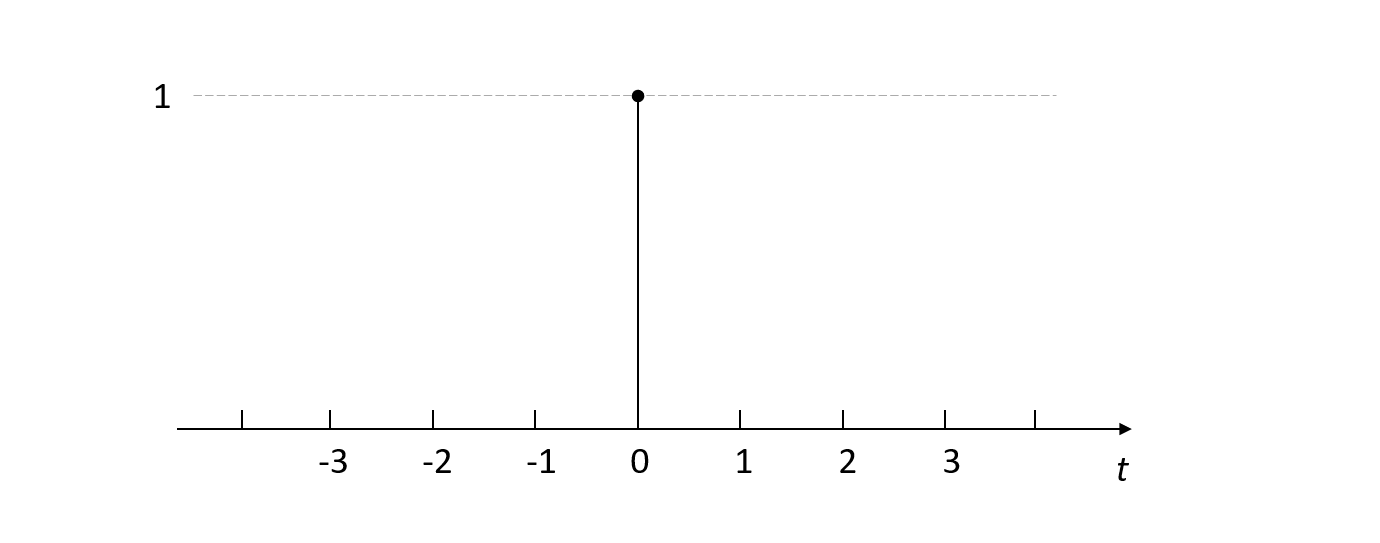
\includegraphics[scale=0.4]{1.png}
    \caption{$\delta $ 函数信号形式}
\end{figure}
\[  \delta [ k] =\left\{ \begin{array}{rcl}
    1 & & {k =0}\\
    0 & & {k\in Z}\\
    \end{array} \right. \]
该函数表现形式被称为$\delta$函数\par
(2) \; 信号用$\delta$函数可以表示为:\par
$f(t)=[ 1,2,3,2,1]  $ \par
\qquad $=f[0]\times \delta [ k]  $ \quad \;  $+$\par
\qquad \quad $ f[1]\times \delta [ k-1]  $  $+$\par
\qquad \quad $ f[2]\times \delta [ k-2]  $  $+$\par
\qquad \quad $ f[3]\times \delta [ k-3]  $  $+$\par
\qquad \quad $ f[4]\times \delta [ k-4]  $  \par
思考:除了$\delta$函数是否还有其他的 Basic signal ,如何用它们表示复杂信号?是否比$\delta$函数好?哪些是我们想要用的 Basic signal?哪些是我们不想用的?\par
(3) \; 用一般信号表示特殊信号 \par
任意信号都可以用冲激信号的组合表示\par
对于离散信号:\par
\[ f[ k] =\sum_{\tau =-\infty}^{\infty} f[\tau  ]\cdot \delta [ k-\tau ]    \]\par
对于连续信号:\par
\[ f(t) =  \int_{\tau =-\infty}^{\infty} f(\tau )\cdot \delta (t-\tau  ) \,d\tau    \]
\; \par
\; \par
(4) \; 卷积 \par
\[ f(t)\ast h(t) =  \int_{\tau =-\infty}^{\infty} f(\tau )\cdot h (t-\tau  ) \,d\tau  \]\par
Q1:(3)与(4)中的公式有什么联系,卷积的定义是怎么推导的?\par
对于 LTI 系统:\par
\[ \delta [ k] \longrightarrow h [ k]  \]\par
则有:\par
\[ \sum_{\tau =-\infty}^{\infty} f[\tau  ]\cdot \delta [ k-\tau ] \longrightarrow \sum_{\tau =-\infty}^{\infty} f[\tau  ]\cdot h [ k-\tau ]  \]\par
连续信号同理可表达为:\par
\[ y(t)=f(t)\ast h(t) =  \int_{\tau =-\infty}^{\infty} f(\tau )\cdot h (t-\tau  ) \,d\tau \]\par

\subsection{$\delta $函数连续时的定义}
\[  \delta [ t] =\left\{ \begin{array}{rcl}
    +\infty & & {t=0}\\
    0 & & {e,e}\\
    \end{array} \right. \]
即:\par
\[ \int_{-\infty}^{\infty}\delta (t)  \,dt=1 \]
$\delta $函数连续时称为“dirac delta function”\par
\begin{figure}[h]
    \centering         %使图片居中放置
    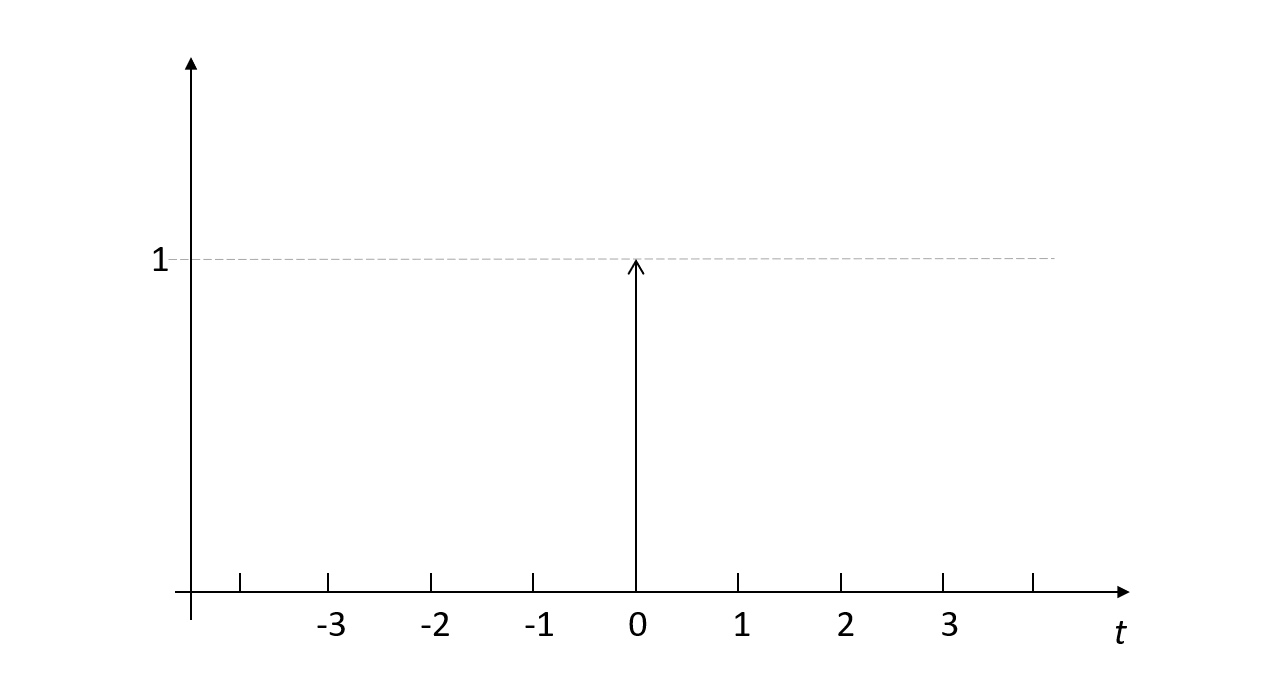
\includegraphics[scale=0.4]{2.png}
    \caption{连续$\delta $ 函数信号表示形式}
\end{figure}
\end{document}